\label{sec:bckgdestimation}

\subsection{\mjj\xspace binning in the resonance analyses}

The \mjj\ bin size is optimized to minimize JER effects, following the studies
performed for the 2015 dijet analysis \cite{EXOT-2015-02} and the Run 2 dijet analysis \cite{Nishu:2646455}.

The following \mjj\ binning is used, which is the same used in the prior Run-2 analyses:
bins = [ 946, 976, 1006, 1037, 1068, 1100, 1133, 1166, 1200, 1234, 1269, 1305, 1341, 1378, 1416, 1454, 1493, 1533, 1573, 1614, 1656, 1698, 1741, 1785, 1830, 1875, 1921, 1968, 2016, 2065, 2114, 2164, 2215, 2267, 2320, 2374, 2429, 2485, 2542, 2600, 2659, 2719, 2780, 2842, 2905, 2969, 3034, 3100, 3167, 3235, 3305, 3376, 3448, 3521, 3596, 3672, 3749, 3827, 3907, 3988, 4070, 4154, 4239, 4326, 4414, 4504, 4595, 4688, 4782, 4878, 4975, 5074, 5175, 5277, 5381, 5487, 5595, 5705, 5817, 5931, 6047, 6165, 6285, 6407, 6531, 6658, 6787, 6918, 7052, 7188, 7326, 7467, 7610, 7756, 7904, 8055, 8208, 8364, 8523, 8685, 8850, 9019, 9191, 9366, 9544, 9726, 9911, 10100, 10292, 10488, 10688, 10892, 11100, 11312, 11528, 11748, 11972, 12200, 12432, 12669, 12910, 13156 ] ~\GeV\. \\

%%%%%%%%%%%%%%%%%%%%%%%%%%%%%%%%%%%%%%%%%%%%%%%%%%%%%%%%%%%%%%%%%%%%
\subsection{Resonance Analysis: Sliding Window Fit (SWiFt)}
%%%%%%%%%%%%%%%%%%%%%%%%%%%%%%%%%%%%%%%%%%%%%%%%%%%%%%%%%%%%%%%%%%%%
In the resonant search the SM background of the \mjj\ spectrum is determined by a functional fit to the data.
Previous searches, from ATLAS and other experiments (such as Refs.~\cite{Bagnaia:1984ip,PhysRevD.79.112002,EXOT-2010-01,CMS-EXO-10-010,EXOT-2010-07,EXOT-2013-11})
have found that a parametric function of the form
\begin{equation}
  f(x) = p_1 (1 - x)^{p_2} x^{p_3 + p_4\ln x + p_5 (\ln x)^2},
\label{Eq:fitfunction}
\end{equation}
where $x \equiv \mjj /\sqrt{s}$, accurately describes dijet mass distribution predicted by leading and next-to-leading-order QCD Monte Carlo.
In the ATLAS 2015 analysis with 3.57~\ifb\ of data the three parameter ($p_4, p_5 = 0$) function sufficiently described the data, while the previous paper publication with 37.0~\ifb\ of data, the four parameter version of the function was found to properly describe the QCD background.  Experience with past experiments has shown that with increased statistics require more and more parameters to properly describe the full invariant mass spectrum.

In a effort to prevent the possible breakdown of our fit function with a high integrated luminosity, the global function fit has been replaced by the Sliding Window Fit method (SWiFt), replacing a fit on the full spectrum with a sliding localized fit on smaller \mjj~ ranges where we expect the function in Equation \ref{Eq:fitfunction} to properly model the QCD background contribution even with very high statistics.  This approach was used in the previous dijet search\cite{EXOT-2016-21}, where the results were cross-checked against the four-parameter global fit function, and in the higher-statistics TLA dijet search \cite{Nishu:2646455}.  SWiFt produces a non-parametric global background model that can be used to search for excesses in the mass spectrum, and to provide inputs to HistFitter to assess limits on specific benchmark signal models.

The methodology behind the SWiFt method is described in \cite{Sekhon:2305523}.

\subsubsection{SWiFt Background}
\label{sec:SwiftBkg}
%%%%%%%%%%%%%%%%%%%%%%%%%%%%%%%%%%%%%%%%%%%%%%%%%%%%%%%%%%%%%%%%%%%%

The SWiFt background is extracted from the data by fitting it using an analytic function. In smaller mass windows, the function is fit to the data and the evaluation of the function at the window's center bin is taken to be the background estimation for the bin. By sliding over the entire mass range, the background is created this way bin-by-bin.  The window size, defined in terms of the window half-width, or the number of mass bins to the left and right of a window center, is chosen to be the largest possible window which satisfies two statistical measures.

The determination of the window size begins with a window half-width of 24 bins, making the window slightly larger than half of the expected invariant mass spectrum for the signal regions, and in line with the window size used in the previous 37.0~\ifb\ iteration of the search.  The sliding window fit procedure is then performed using a four-parameter version of Eq.~\ref{Eq:fitfunction}.  The quality of the fit to the data is considered to be good if it passes two metrics which confirm that the individual windows as well as the global fit describe the data well:

\begin{itemize}
	\item Global $\chi^2$ $p$-value > 0.05
	\item \BumpHunter\ $p$-value > 0.01
\end{itemize}

If these criteria are both met for the window size and fit function, the
background is selected for use in the limit machinery.  If it fails either one
of these metrics, the SWiFt method evolves until a fit which satisfies both
metrics is found.  First, the 5-parameter version of Eq.~\ref{Eq:fitfunction} is
used instead of the 4-parameter version and the fit is re-run.  If this fit also
fails the criteria, the window half-width is reduced by 2 (thus, the whole
window shrinks by four bins) and the fit is repeated with the 4-parameter
function.  This process of alternating between increasing the number of
parameters in the fit function and reducing the number of parameters and
shrinking the window size is repeated until a satisfactory fit is obtained.
Exception to this rule applies if the \BumpHunter~ $p$-value indicates a signal.
In this case, the S+B fit is repeated to asses the level of compatibility with
the model when considering full systematical uncertainty.

The difference between the nominal background (using the n-parameter function) and the alternate background (using the n+1 parameter function) will later be assessed as a systematic uncertainty.

\todo[inline]{Need to  check SWiFt with gluon selection applied. Update for new pseudo-data method.} 
{\textit {\textcolor{red}{ The background making procedure has been validated using pseudo-data sets derived from the nominal SWiFt background. While ideally this would be performed on MC, its limited statistics compared to the data prevent any useful conclusions from being drawn. Several pseudo-data sets have been evaluated by taking the fit result from the 2015+2016 data (37\ifb), scaling up to the expected full Run-2 dataset, Poisson-fluctuating the background to obtain a data-like spectrum, and running the fit procedure over this pseudo-data set.  This procedure has shown that the starting function can be reasonably expected to perform well for the full Run-2 dataset.}}}


The background-only hypothesis is used as input to \BumpHunter\,  which
identifies if there is a significant excess in the data.

If \BumpHunter\ shows good compatibility between the data and the
background-only hypothesis (\BumpHunter\ p-value larger than 0.01) the exclusion
limits are set. A S+B fit is run for different signal hypotheses. The signal template at each mass window
is determined by the morphing procedure described in

\subsection{Pseudo-data for Validation}
\label{sec:pseudo}

Pseudo-data for finding and validating the optimal gluon selection is created using the 
\todo{Check that using good fit to full data with appropriate settings} 
SWiFt fit result from the full Run 2 dataset scaled with the smoothed 
fraction of events that pass the selection criteria in the simulated \QCD\  dataset. 
The SWiFt fit used in the creation of the pseudo-data is shown in Fig.~\ref{fig:SWiFt_Run2}.

The fraction of \QCD\ events that pass the gluon-gluon selection criteria is smoothed
using Friedman's `super smoother' with maximum smoothness. The choice of smoother is not 
very important as the 
fraction changes slowly over a small range. The fraction for a gluon-gluon selection efficiency of 
75\% per jet the fraction runs from 27\% at 1.1\,\TeV\ to 13\% at 8\,\TeV\ (Fig.~\ref{fig:Smoothed_GG_Fraction}).

\begin{figure}[htb]
 \centering
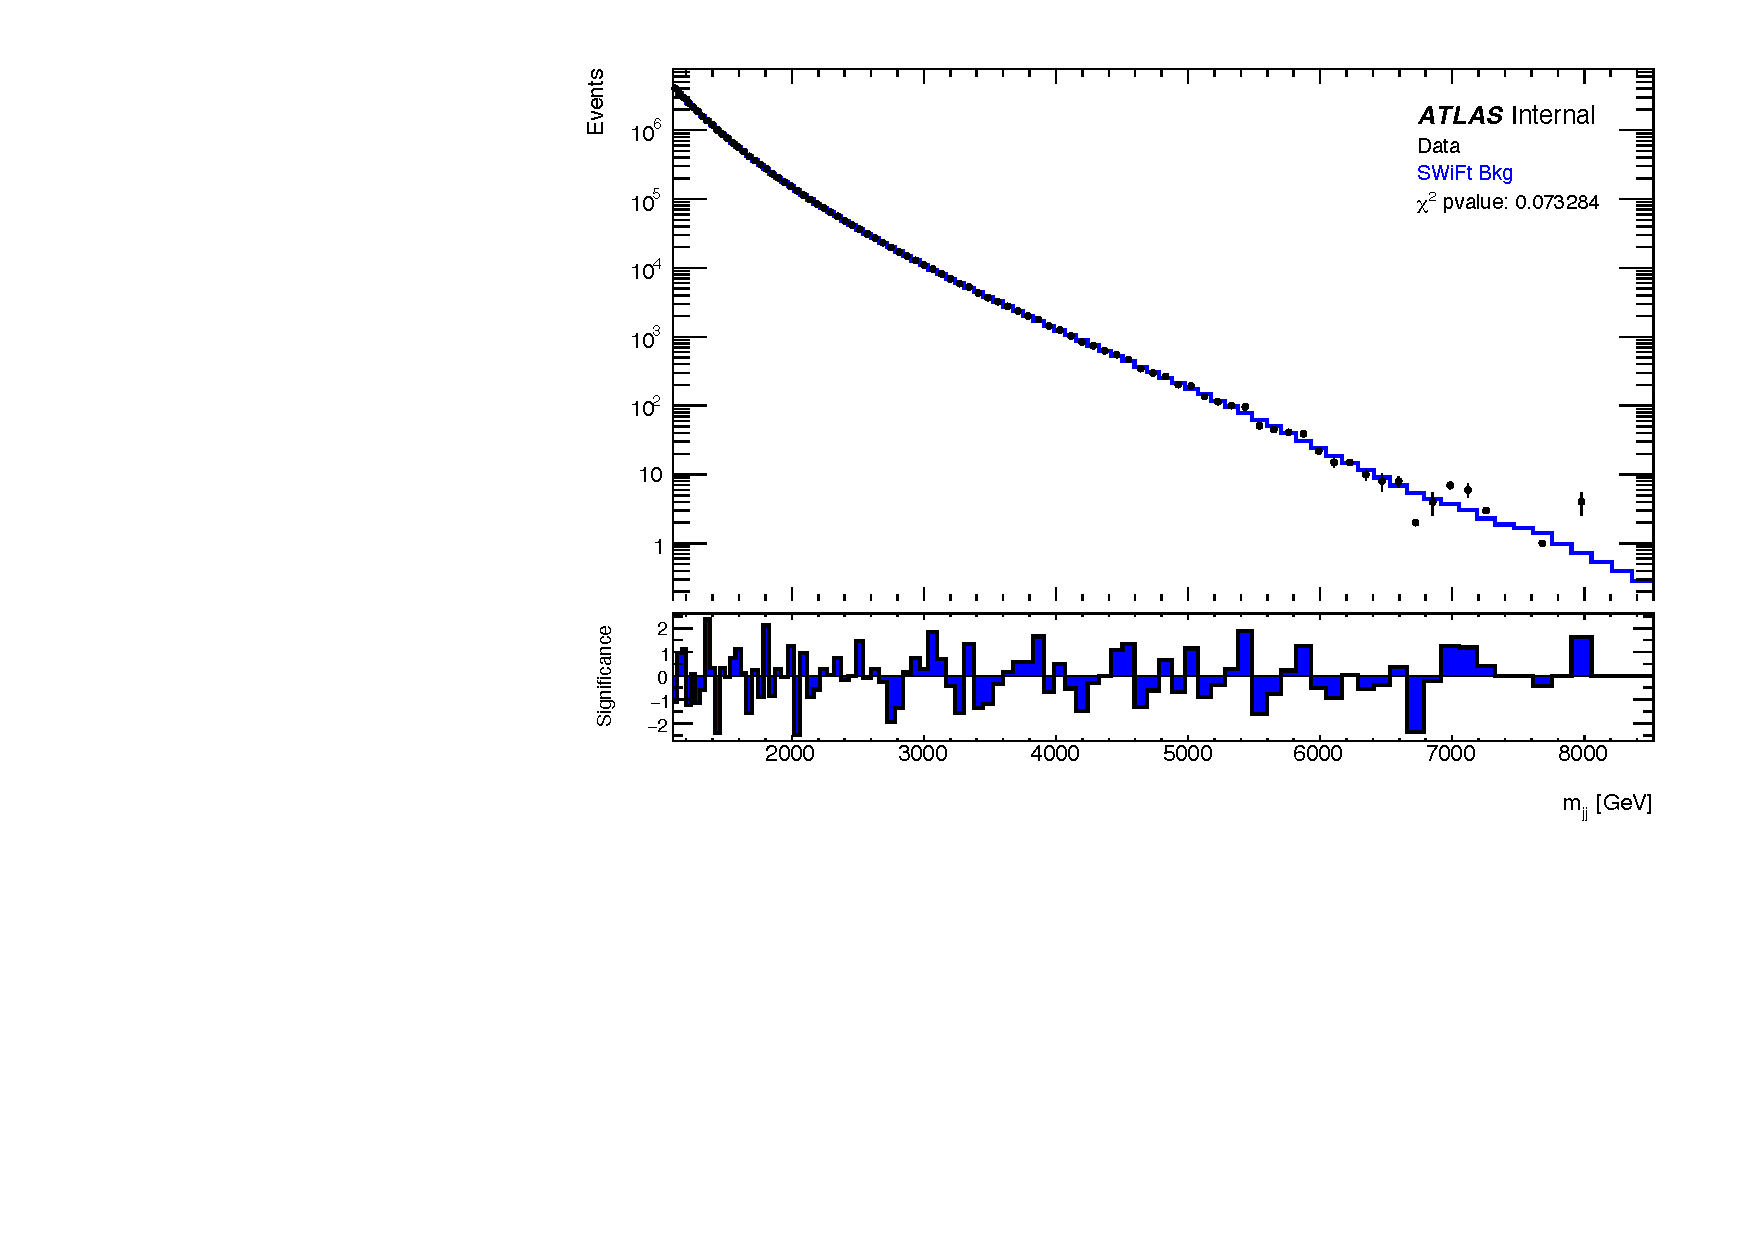
\includegraphics[width=0.75\textwidth]{figures/04-BackgroundEstimation/SWiFtData15-18.pdf}
\caption{SWiFt fit to the Run 2 data set used for creating pseudo-data.  \label{fig:SWiFt_Run2}}
\end{figure}

\begin{figure}[htb]
 \centering
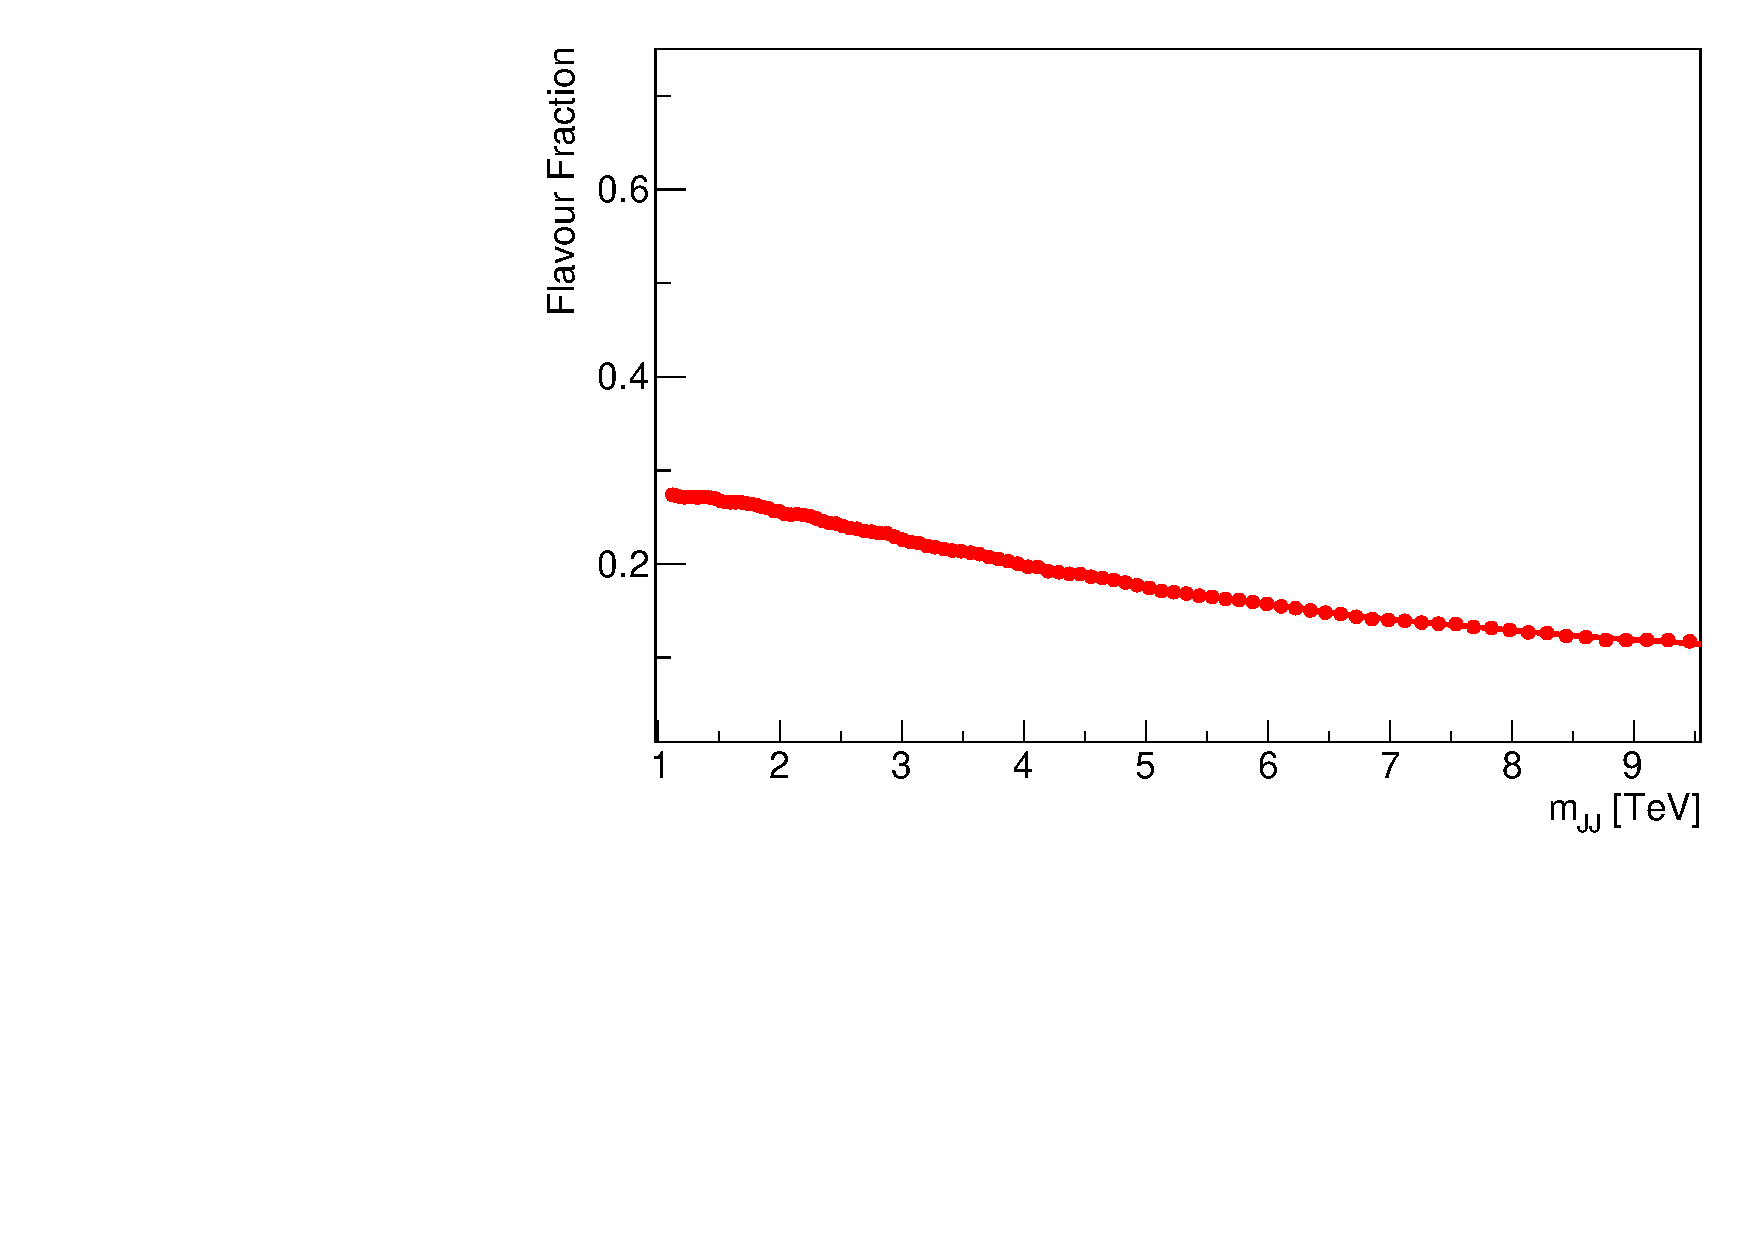
\includegraphics[width=0.75\textwidth]{figures/04-BackgroundEstimation/fracSmoothSelected_GG_New_Selection5.pdf}
\caption{The smoothed fraction of events that pass gluon selection with 75\% efficiency.   \label{fig:Smoothed_GG_Fraction}}
\end{figure}

An example of a pseudo-data set created with a gluon efficiency of 75\% having been run through SWiFt and \BumpHunter\ 
is shown in Figures~\ref{fig:SWiFtPD_75percentGG} and \ref{fig:figure1_GG_PD_75percent} showing that SWiFt 
does a good job of fitting the gluon selected background distribution. 


\begin{figure}[htb]
 \centering
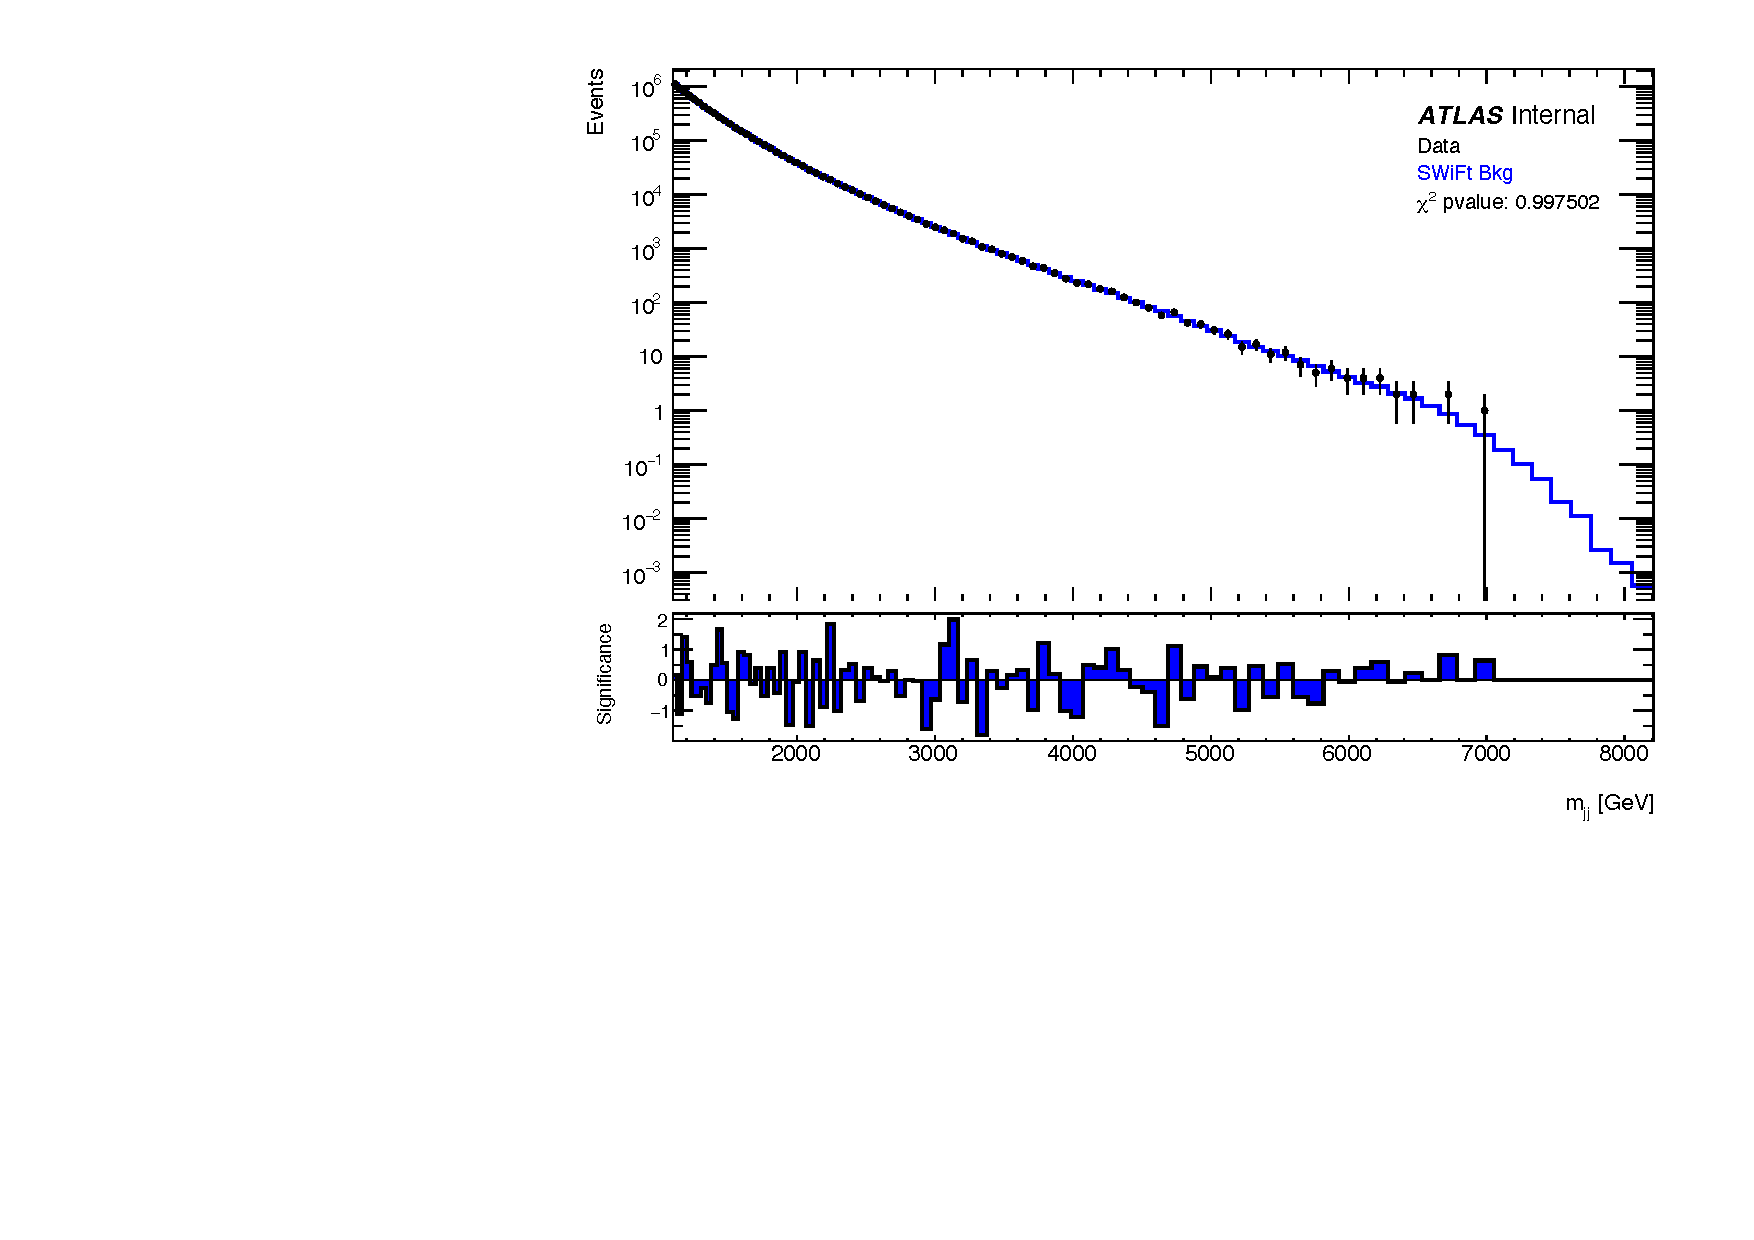
\includegraphics[width=0.75\textwidth]{figures/04-BackgroundEstimation/SWiFtPD_75percentGG}
\caption{SWiFt fit pseudo-data for a two gluon selection with 75\% efficiency.  \label{fig:SWiFtPD_75percentGG}}
\end{figure}


\begin{figure}[htb]
 \centering
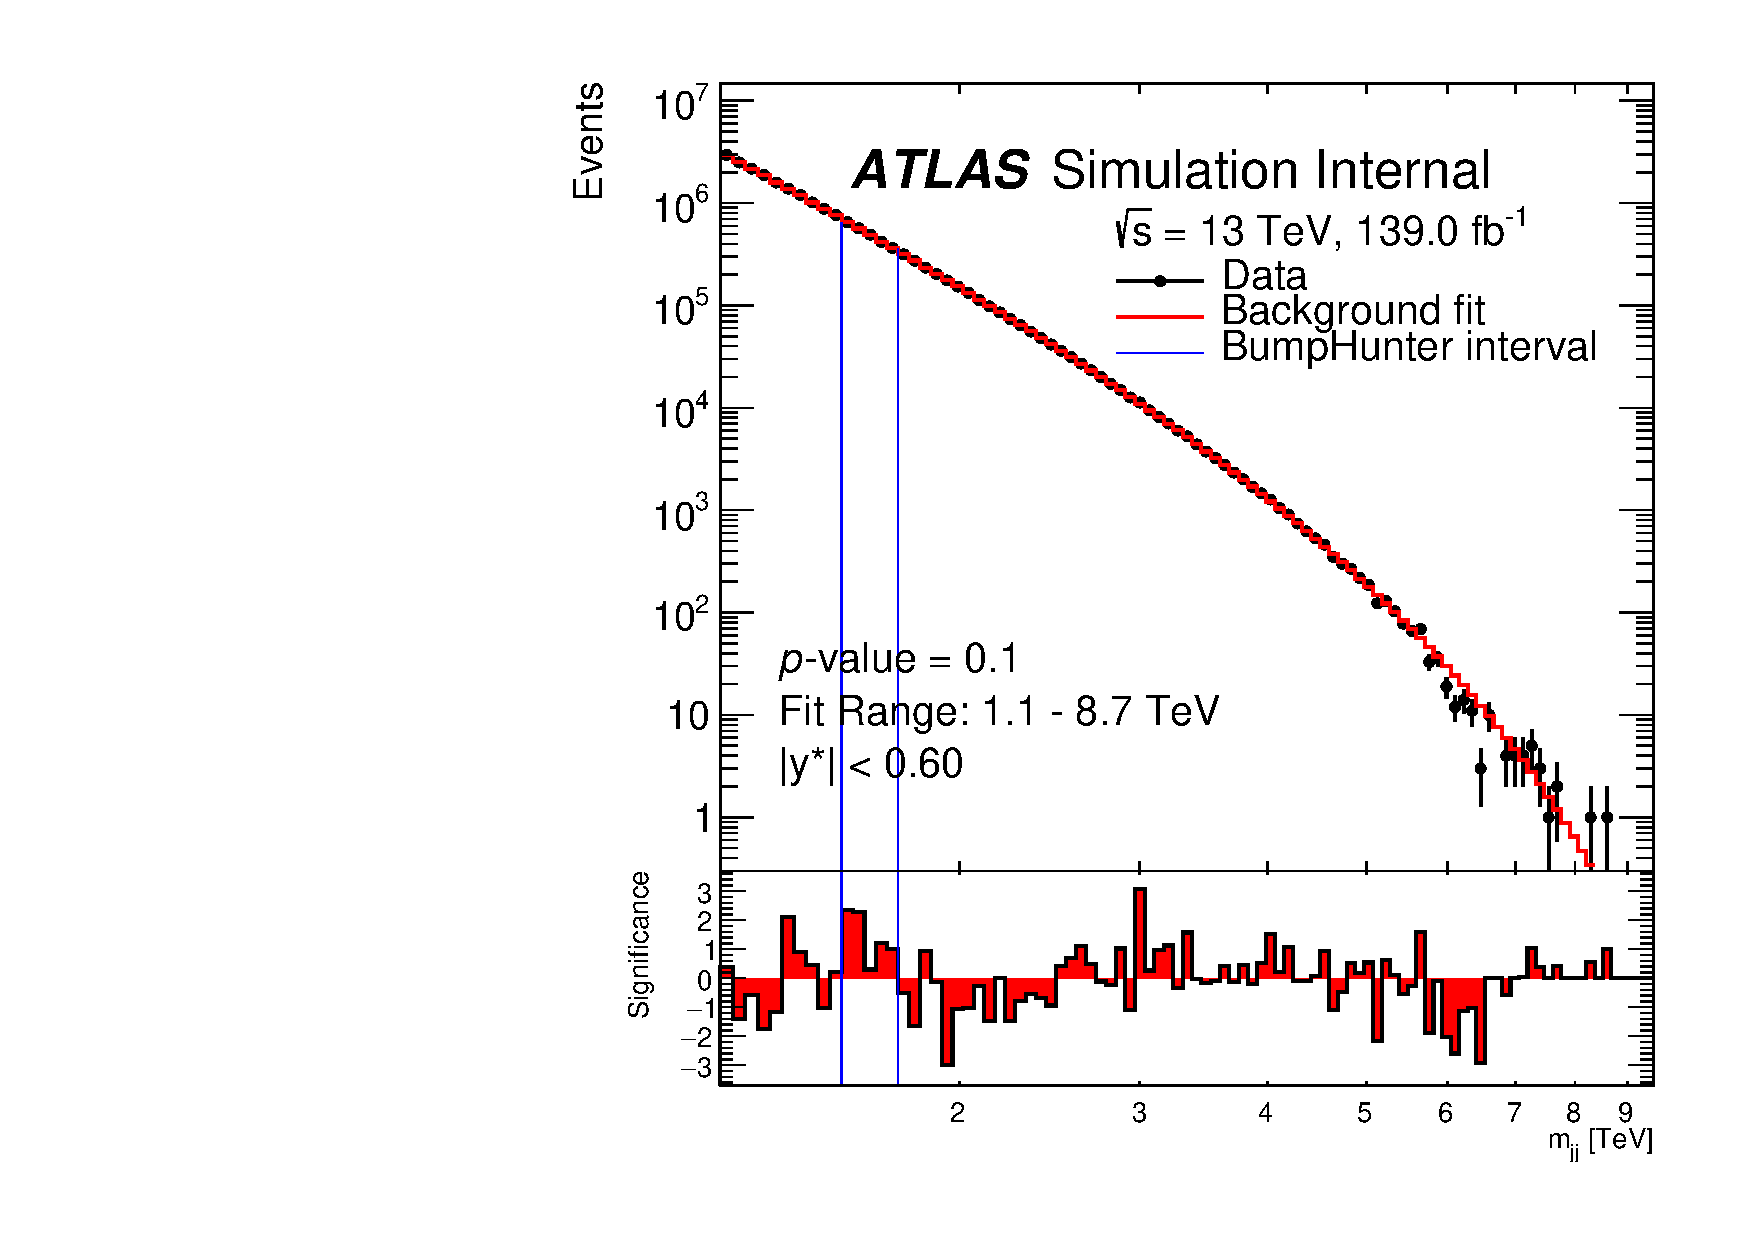
\includegraphics[width=0.75\textwidth]{figures/04-BackgroundEstimation/figure1_GG_PD_75percent.pdf}
\caption{\BumpHunter\ run on a pseudo-data for a two gluon selection with 75\% efficiency.\label{fig:figure1_GG_PD_75percent}}
\end{figure}

